Consensus is formed on state register transformations.

Ledgers are defined by policies stipulating the consensus networks they recognise. Inter-ledger operations require only mutual recognition of consensus networks.

Ledgers as oracles.

Finite state machine oracles.

The combined public broadcasts across all networks acts as a global oracle for ledger states, facilitating a high arbitrage environment in an algorithmic context, an equilibrating force across the ledgers of parallel markets or interconnected markets.

Inter-ledger transactions require only mutual recognition of consensus, defined by the networks from which they are drawn.

* Sec: ledger transaction queues.

* Hierarchical bidding to maximise resource utilisation.

* Subsection: blockchains.
%\subsection{Blockchains}

Blockchains are protocol-level applications for consensus, following their own rules on what consensus is formed on. A blockchain's transaction history is immutable and may be retrospectively evaluated. Blockchain implementations typically consider asynchronous operating environments. In this setting simultaneous block additions manifest themselves as forks, requiring error correction mechanisms to maintain the integrity of the chain. Formally, a pool of valid block additions defines a directed tree graph which the blockchain implementation must correct to a directed linear graph.

In a synchronous setting where a ledger is associated with consensus derived from a given network these considerations change. Rather than performing consensus assignment on the basis of unique transaction identifiers we assign on the basis of transaction queue identifiers associated with individual ledgers. From the pool of accepted bids nodes assigned to a given transaction queue consensus set process all bids associated with that queue, batch processed in accordance with the ledger's transaction amalgamation rules. Employing queue assignment rather than transaction assignment mitigates the possibility of fork formation. In a proof-of-work setting this issue may be addressed by introducing friction. However, while this hinders double-mining it also undermines transaction processing rates, an undesirable tradeoff.

If $n$ consensus sets of size $N$ independently form honest majority their union of size $nN$ necessarily forms honest majority. Hence,
\begin{align}
	P(nN,r)\leq\varepsilon \,\Rightarrow\, P(N,r)^n\leq\varepsilon.
\end{align}
For $n=1$ this reduces to consensus by majority vote amongst $N$ parties, while the opposing limiting case of $n=N$ reduces to consensus by unanimity amongst $N$ parties. A blockchain with unanimous $n$-level retrospective verification affords $\varepsilon^n$-security, and the associated tradeoff in required consensus set size scales as,
\begin{align}
	N_\mathrm{min}(r,\varepsilon) = N_\mathrm{min}^{(n)}(r,\varepsilon^n),
\end{align}
which implies,
\begin{align}
	P_c(N,r) = P_c(N^{(n)},r)^n.
\end{align}

Now $\varepsilon$ represents the effective error rate in new block additions while \mbox{$\varepsilon'=\varepsilon^n$} is the effective security parameter which applies only to blocks at least $n$ steps back, which have been subject to $n$ independent verifications. These blocks are considered \emph{complete} whereas more recent blocks are considered \emph{pending}, potentially still subject to being invalidated (Fig.~\ref{fig:backward_integrity}). Only the most recent \emph{complete} block must persist to maintain the blockchain, the point to which the blockchain is reverted if \emph{pending} blocks are invalidated.

\begin{figure}[!htb]
	\begin{tikzpicture}[genericStyle, scale=0.5]
  \def\myWidth{6em}
  \def\myHeight{2.5em}

  \fill[fill=topologyFillColor] (-\myWidth,0) rectangle (\myWidth,10.5);

  \node[draw=none, fill=cyan!20, ellipse, minimum width=\myWidth, minimum height=\myHeight, fill=blockchainDiscColor, myShadow] (node0) at (0,0) {$\varepsilon^n$};
  \node[draw=none, ellipse, minimum width=\myWidth, minimum height=\myHeight, fill=blockchainDiscColor] (node1) at (0,3.5) {$\varepsilon^n$};
  \draw[darkgray] (-\myWidth,3.5) arc [start angle=0, end angle=-180, x radius=-\myWidth, y radius =\myHeight];
  \draw[gray, dashed] (-\myWidth,3.5) arc [start angle=0, end angle=180, x radius=-\myWidth, y radius =\myHeight];

  \node[draw=none, ellipse, minimum width=\myWidth, minimum height=\myHeight, fill=blockchainPendingDiscColor] (node2) at (0,5) {$\varepsilon^n$};
  \draw[darkgray] (-\myWidth,5) arc [start angle=0, end angle=-180, x radius=-\myWidth, y radius =\myHeight];
  \draw[gray, dashed] (-\myWidth,5) arc [start angle=0, end angle=180, x radius=-\myWidth, y radius =\myHeight];

  \node[draw=none, ellipse, minimum width=\myWidth, minimum height=\myHeight, fill=blockchainPendingDiscColor] (node3) at (0,7) {$\varepsilon^{n-1}$};
  \draw[darkgray] (-\myWidth,7) arc [start angle=0, end angle=-180, x radius=-\myWidth, y radius =\myHeight];
  \draw[gray, dashed] (-\myWidth,7) arc [start angle=0, end angle=180, x radius=-\myWidth, y radius =\myHeight];

  \draw[darkgray] (-\myWidth,0) arc [start angle=0, end angle=-180, x radius=-\myWidth, y radius =\myHeight];
  \draw[gray, dashed] (-\myWidth,0) arc [start angle=0, end angle=180, x radius=-\myWidth, y radius =\myHeight];

  \node[draw=none] (node4) at (0,2) {$\vdots$};
  \node[draw=none] (node4) at (0,9) {$\vdots$};
  \node[darkgray, ellipse, minimum width=\myWidth, minimum height=\myHeight, fill=blockchainPendingDiscColor] (node5) at (0,10.5) {$\varepsilon$};

  \draw (-\myWidth,0) -- (-\myWidth,10.5);
  \draw (\myWidth,0) -- (\myWidth,10.5);

  \coordinate (ltop) at ($(node5.west) + (-2em,0)$);
  \coordinate (lbot) at ($(node2.west) + (-2em,0)$);
  \coordinate (backC) at ($(ltop.west)!0.5!(lbot.west) + (-1.2em,0)$);

  \coordinate (pendtop) at ($(node5.east) + (2em,\myHeight)$);
  \coordinate (pendbot) at ($(node2.east) + (2em,0)$);
  \coordinate (pendtopin) at ($(pendtop) + (-0.5em,0)$);
  \coordinate (pendbotin) at ($(pendbot) + (-0.5em,0)$);
  \coordinate (pendC) at ($(pendbot)!0.5!(pendtop) + (1.5em,0)$);

  \coordinate (comptop) at ($(node1.east) + (2em,\myHeight)$);
  \coordinate (compbot) at ($(node0.east) + (2em,-\myHeight)$);
  \coordinate (comptopin) at ($(comptop) + (-0.5em,0)$);
  \coordinate (compC) at ($(compbot)!0.5!(comptop) + (1.5em,0)$);

  \draw[darkgray, <->, thick] (ltop) -- (lbot);
  \draw[redHighlightColor, thick] (pendtopin) -- (pendtop) -- (pendbot) -- (pendbotin);
  \draw[->, blueHighlightColor, thick] (comptopin) -- (comptop) -- (compbot);

  \node[draw=none, rotate=90, text=red] at (pendC) {pending};
  \node[draw=none, rotate=90, text=blue] at (compC) {complete};
  \node[draw=none, text=black] at (backC) {$n$};
\end{tikzpicture}
	\caption{\textbf{Blockchain with $n$-level reverse integrity checking.} Upon addition of the top-level block consensus requires verifying integrity going back $n$ blocks. If consensus has $\varepsilon$-security, for $i\leq n$ the $i$th past block will have been verified $i$ times, exhibiting cumulative $\varepsilon^i$-security. Blocks $i\geq n$ all exhibit $\varepsilon'=\varepsilon^n$ integrity, the security parameter of the blockchain. The $\varepsilon$-security of the top block may be interpreted as the effective error rate in block addition, where error correction is implemented at the blockchain's protocol level.} \label{fig:backward_integrity}
\end{figure}

\begin{figure}[!htb]
	\centering
	\resizebox{\columnwidth}{!}{
\begin{tikzpicture}
\begin{axis}[
    xlabel={$\varepsilon$},
    ylabel={$\varepsilon'$},
    xmin=0, xmax=1,
    ymin=0, ymax=1,
    restrict y to domain=0:1,
    grid style=dashed,
    xtick={0, 1},
    ytick={0, 1}, 
    ylabel style={rotate=-90, xshift=1.2em},
    xlabel style={yshift=1.2em},
    unit vector ratio=5 3,
]

% Plot x
\addplot[
    color=blue,
    domain=0:1,
    samples=200,
    line width=1pt,
    ]
    {x};

% Plot x^2
\addplot[
    color=orange,
    domain=0:1,
    samples=200,
    line width=1pt,
    ]
    {x^2};

% Plot x^3
\addplot[
    color=green,
    domain=0:1,
    samples=200,
    line width=1pt,
    ]
    {x^4};
% \addlegendentry{$x^4$}

\node at (axis cs:0.2,0.8) {\parbox{4cm}{
        \begin{align*}
            &n = 1\\
            &\varepsilon'=\varepsilon\\
            &\mathrm{cost}=N\\
            &\textsc{MajorityVote}
        \end{align*}
    }};

\node at (axis cs:0.8,0.2) {\parbox{4cm}{
        \begin{align*}
            n = N\\
            \varepsilon'=r\\
            \mathrm{cost}=1\\
            \textsc{UnanimousVote}
        \end{align*}
    }};


\end{axis}
\end{tikzpicture}
}
%	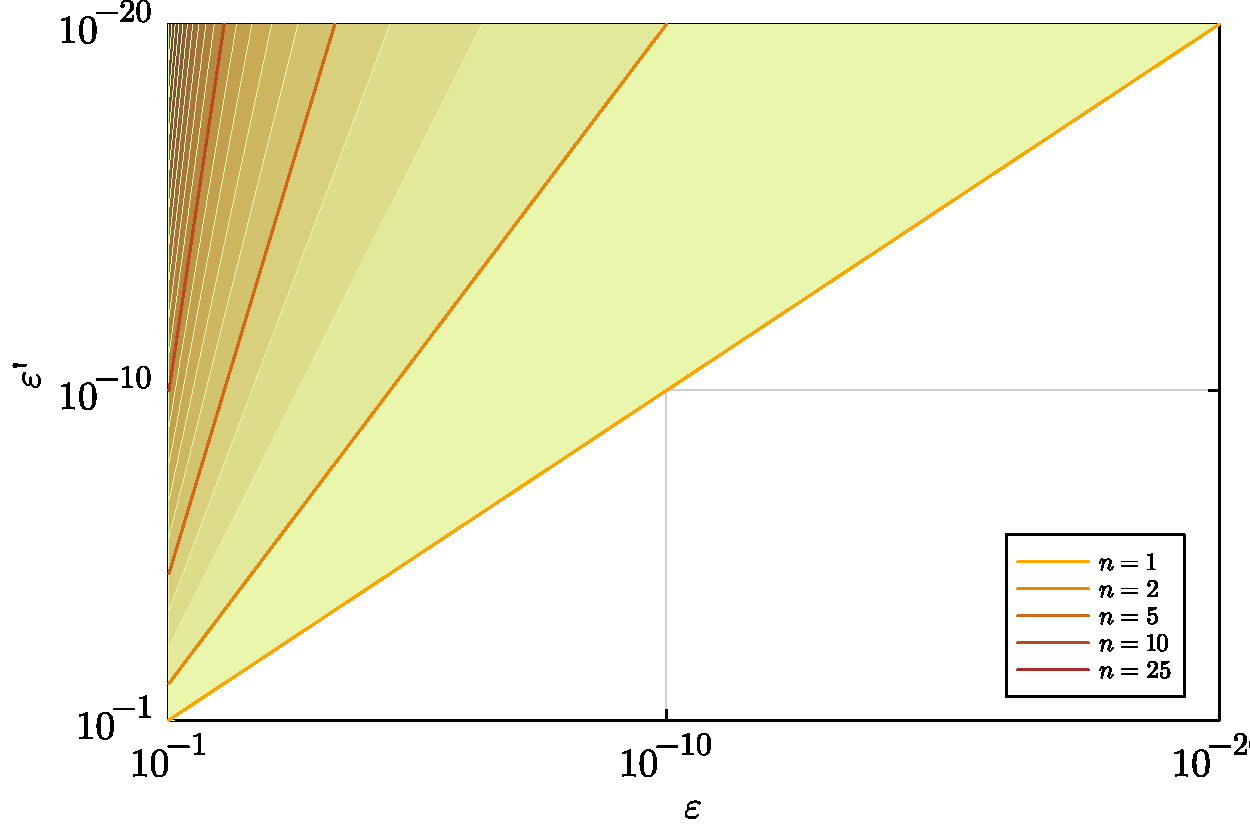
\includegraphics[width=\columnwidth]{figs/blockchain_security_tradeoff.pdf}
	\caption{\textbf{Tradeoffs in blockchain integrity with retrospective consensus verification. ??? TODO}}\label{fig:blockchain_security_tradeoff}
\end{figure}